\documentclass[twoside]{book}

% Packages required by doxygen
\usepackage{fixltx2e}
\usepackage{calc}
\usepackage{doxygen}
\usepackage[export]{adjustbox} % also loads graphicx
\usepackage{graphicx}
\usepackage[utf8]{inputenc}
\usepackage{makeidx}
\usepackage{multicol}
\usepackage{multirow}
\PassOptionsToPackage{warn}{textcomp}
\usepackage{textcomp}
\usepackage[nointegrals]{wasysym}
\usepackage[table]{xcolor}

% Font selection
\usepackage[T1]{fontenc}
\usepackage[scaled=.90]{helvet}
\usepackage{courier}
\usepackage{amssymb}
\usepackage{sectsty}
\renewcommand{\familydefault}{\sfdefault}
\allsectionsfont{%
  \fontseries{bc}\selectfont%
  \color{darkgray}%
}
\renewcommand{\DoxyLabelFont}{%
  \fontseries{bc}\selectfont%
  \color{darkgray}%
}
\newcommand{\+}{\discretionary{\mbox{\scriptsize$\hookleftarrow$}}{}{}}

% Page & text layout
\usepackage{geometry}
\geometry{%
  a4paper,%
  top=2.5cm,%
  bottom=2.5cm,%
  left=2.5cm,%
  right=2.5cm%
}
\tolerance=750
\hfuzz=15pt
\hbadness=750
\setlength{\emergencystretch}{15pt}
\setlength{\parindent}{0cm}
\setlength{\parskip}{3ex plus 2ex minus 2ex}
\makeatletter
\renewcommand{\paragraph}{%
  \@startsection{paragraph}{4}{0ex}{-1.0ex}{1.0ex}{%
    \normalfont\normalsize\bfseries\SS@parafont%
  }%
}
\renewcommand{\subparagraph}{%
  \@startsection{subparagraph}{5}{0ex}{-1.0ex}{1.0ex}{%
    \normalfont\normalsize\bfseries\SS@subparafont%
  }%
}
\makeatother

% Headers & footers
\usepackage{fancyhdr}
\pagestyle{fancyplain}
\fancyhead[LE]{\fancyplain{}{\bfseries\thepage}}
\fancyhead[CE]{\fancyplain{}{}}
\fancyhead[RE]{\fancyplain{}{\bfseries\leftmark}}
\fancyhead[LO]{\fancyplain{}{\bfseries\rightmark}}
\fancyhead[CO]{\fancyplain{}{}}
\fancyhead[RO]{\fancyplain{}{\bfseries\thepage}}
\fancyfoot[LE]{\fancyplain{}{}}
\fancyfoot[CE]{\fancyplain{}{}}
\fancyfoot[RE]{\fancyplain{}{\bfseries\scriptsize Generated by Doxygen }}
\fancyfoot[LO]{\fancyplain{}{\bfseries\scriptsize Generated by Doxygen }}
\fancyfoot[CO]{\fancyplain{}{}}
\fancyfoot[RO]{\fancyplain{}{}}
\renewcommand{\footrulewidth}{0.4pt}
\renewcommand{\chaptermark}[1]{%
  \markboth{#1}{}%
}
\renewcommand{\sectionmark}[1]{%
  \markright{\thesection\ #1}%
}

% Indices & bibliography
\usepackage{natbib}
\usepackage[titles]{tocloft}
\setcounter{tocdepth}{3}
\setcounter{secnumdepth}{5}
\makeindex

% Hyperlinks (required, but should be loaded last)
\usepackage{ifpdf}
\ifpdf
  \usepackage[pdftex,pagebackref=true]{hyperref}
\else
  \usepackage[ps2pdf,pagebackref=true]{hyperref}
\fi
\hypersetup{%
  colorlinks=true,%
  linkcolor=blue,%
  citecolor=blue,%
  unicode%
}

% Custom commands
\newcommand{\clearemptydoublepage}{%
  \newpage{\pagestyle{empty}\cleardoublepage}%
}

\usepackage{caption}
\captionsetup{labelsep=space,justification=centering,font={bf},singlelinecheck=off,skip=4pt,position=top}

%===== C O N T E N T S =====

\begin{document}

% Titlepage & ToC
\hypersetup{pageanchor=false,
             bookmarksnumbered=true,
             pdfencoding=unicode
            }
\pagenumbering{alph}
\begin{titlepage}
\vspace*{7cm}
\begin{center}%
{\Large M\+I\+D\+I\+Analyzer }\\
\vspace*{1cm}
{\large Generated by Doxygen 1.8.13}\\
\end{center}
\end{titlepage}
\clearemptydoublepage
\pagenumbering{roman}
\tableofcontents
\clearemptydoublepage
\pagenumbering{arabic}
\hypersetup{pageanchor=true}

%--- Begin generated contents ---
\chapter{Class Index}
\section{Class List}
Here are the classes, structs, unions and interfaces with brief descriptions\+:\begin{DoxyCompactList}
\item\contentsline{section}{\hyperlink{structMIDIBlockStatus}{M\+I\+D\+I\+Block\+Status} }{\pageref{structMIDIBlockStatus}}{}
\end{DoxyCompactList}

\chapter{File Index}
\section{File List}
Here is a list of all documented files with brief descriptions\-:\begin{DoxyCompactList}
\item\contentsline{section}{include/\hyperlink{debug_8h}{debug.\-h} }{\pageref{debug_8h}}{}
\item\contentsline{section}{include/{\bfseries main.\-h} }{\pageref{main_8h}}{}
\item\contentsline{section}{include/{\bfseries midi\-\_\-errors.\-h} }{\pageref{midi__errors_8h}}{}
\item\contentsline{section}{include/{\bfseries midi\-\_\-parse.\-h} }{\pageref{midi__parse_8h}}{}
\item\contentsline{section}{include/{\bfseries midi\-\_\-reader.\-h} }{\pageref{midi__reader_8h}}{}
\item\contentsline{section}{src/\hyperlink{main_8c}{main.\-c} }{\pageref{main_8c}}{}
\item\contentsline{section}{src/\hyperlink{midi__parse_8c}{midi\-\_\-parse.\-c} }{\pageref{midi__parse_8c}}{}
\item\contentsline{section}{src/\hyperlink{midi__reader_8c}{midi\-\_\-reader.\-c} }{\pageref{midi__reader_8c}}{}
\end{DoxyCompactList}

\chapter{Class Documentation}
\hypertarget{structMIDIBlock}{}\section{M\+I\+D\+I\+Block Struct Reference}
\label{structMIDIBlock}\index{M\+I\+D\+I\+Block@{M\+I\+D\+I\+Block}}
\subsection*{Public Attributes}
\begin{DoxyCompactItemize}
\item 
\mbox{\Hypertarget{structMIDIBlock_a02e4e52dba7225c6f89d42dc15446793}\label{structMIDIBlock_a02e4e52dba7225c6f89d42dc15446793}} 
unsigned char {\bfseries header} \mbox{[}4\mbox{]}
\item 
\mbox{\Hypertarget{structMIDIBlock_a33e82a075a2c389e4fb4ec3f863cd0b5}\label{structMIDIBlock_a33e82a075a2c389e4fb4ec3f863cd0b5}} 
int {\bfseries size}
\item 
\mbox{\Hypertarget{structMIDIBlock_a69c7c7dbb87cd8eb4e2821ccc1aef4fb}\label{structMIDIBlock_a69c7c7dbb87cd8eb4e2821ccc1aef4fb}} 
unsigned char $\ast$ {\bfseries data}
\end{DoxyCompactItemize}


The documentation for this struct was generated from the following file\+:\begin{DoxyCompactItemize}
\item 
include/midi\+\_\+reader.\+h\end{DoxyCompactItemize}

\hypertarget{structMIDIBlockStatus}{}\section{M\+I\+D\+I\+Block\+Status Struct Reference}
\label{structMIDIBlockStatus}\index{M\+I\+D\+I\+Block\+Status@{M\+I\+D\+I\+Block\+Status}}
\subsection*{Public Attributes}
\begin{DoxyCompactItemize}
\item 
\mbox{\Hypertarget{structMIDIBlockStatus_a4ff218757771301c23514d2ab31af146}\label{structMIDIBlockStatus_a4ff218757771301c23514d2ab31af146}} 
unsigned char $\ast$ {\bfseries data}
\item 
\mbox{\Hypertarget{structMIDIBlockStatus_af35dc6eeaa93f01c73e308a6d34316d3}\label{structMIDIBlockStatus_af35dc6eeaa93f01c73e308a6d34316d3}} 
int {\bfseries data\+Size}
\item 
\mbox{\Hypertarget{structMIDIBlockStatus_a1db881c91aaf122add746eacb30acebf}\label{structMIDIBlockStatus_a1db881c91aaf122add746eacb30acebf}} 
int {\bfseries is\+Playing}
\item 
\mbox{\Hypertarget{structMIDIBlockStatus_a671d56d5ecea2ed5e94b871e5995c6f1}\label{structMIDIBlockStatus_a671d56d5ecea2ed5e94b871e5995c6f1}} 
int {\bfseries delta\+Ticks}
\item 
\mbox{\Hypertarget{structMIDIBlockStatus_a27dae156bd6248d095ad04d41ef6d4f8}\label{structMIDIBlockStatus_a27dae156bd6248d095ad04d41ef6d4f8}} 
int {\bfseries current\+Pos}
\end{DoxyCompactItemize}


The documentation for this struct was generated from the following file\+:\begin{DoxyCompactItemize}
\item 
src/\hyperlink{main_8c}{main.\+c}\end{DoxyCompactItemize}

\chapter{File Documentation}
\hypertarget{debug_8h}{}\section{include/debug.h File Reference}
\label{debug_8h}\index{include/debug.\+h@{include/debug.\+h}}
{\ttfamily \#include $<$stdio.\+h$>$}\newline
{\ttfamily \#include $<$stdlib.\+h$>$}\newline
{\ttfamily \#include $<$string.\+h$>$}\newline
Include dependency graph for debug.\+h\+:

\hypertarget{main_8c}{}\section{src/main.c File Reference}
\label{main_8c}\index{src/main.\+c@{src/main.\+c}}
{\ttfamily \#include $<$stdio.\+h$>$}\newline
{\ttfamily \#include $<$stdlib.\+h$>$}\newline
{\ttfamily \#include $<$string.\+h$>$}\newline
{\ttfamily \#include $<$errno.\+h$>$}\newline
{\ttfamily \#include $<$fcntl.\+h$>$}\newline
{\ttfamily \#include $<$unistd.\+h$>$}\newline
{\ttfamily \#include $<$time.\+h$>$}\newline
{\ttfamily \#include \char`\"{}main.\+h\char`\"{}}\newline
{\ttfamily \#include \char`\"{}midi\+\_\+reader.\+h\char`\"{}}\newline
{\ttfamily \#include \char`\"{}midi\+\_\+parse.\+h\char`\"{}}\newline
{\ttfamily \#include \char`\"{}debug.\+h\char`\"{}}\newline
Include dependency graph for main.\+c\+:\nopagebreak
\begin{figure}[H]
\begin{center}
\leavevmode
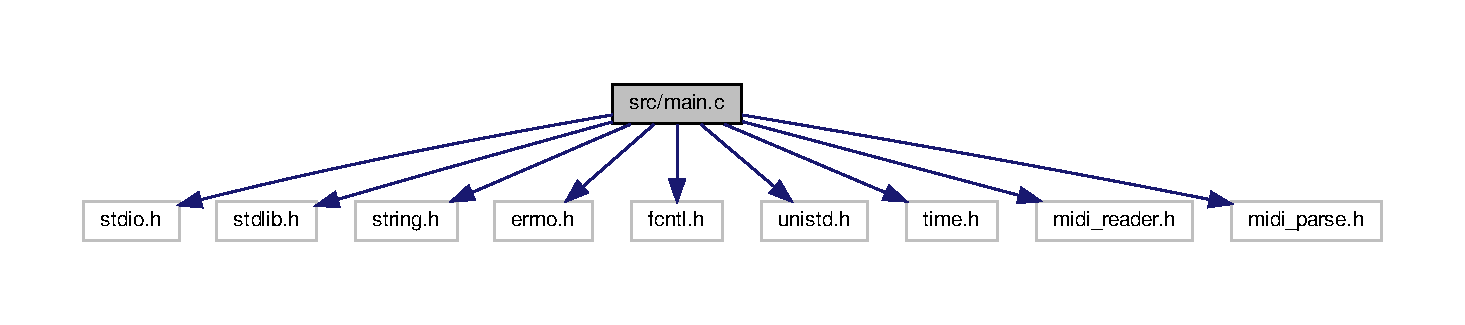
\includegraphics[width=350pt]{main_8c__incl}
\end{center}
\end{figure}
\subsection*{Classes}
\begin{DoxyCompactItemize}
\item 
struct \hyperlink{structMIDIBlockStatus}{M\+I\+D\+I\+Block\+Status}
\end{DoxyCompactItemize}
\subsection*{Functions}
\begin{DoxyCompactItemize}
\item 
\mbox{\Hypertarget{main_8c_adae8c2dcd3d6726f629d7015c30f81ae}\label{main_8c_adae8c2dcd3d6726f629d7015c30f81ae}} 
int {\bfseries M\+I\+D\+I\+Block\+Status\+\_\+is\+Playing} (struct \hyperlink{structMIDIBlockStatus}{M\+I\+D\+I\+Block\+Status} $\ast$midi\+\_\+block\+\_\+status, int count)
\item 
\mbox{\Hypertarget{main_8c_a61bd11e29e619346a057fdb02960b7ef}\label{main_8c_a61bd11e29e619346a057fdb02960b7ef}} 
int {\bfseries M\+I\+D\+I\+Block\+Status\+\_\+update\+Delta\+Time} (struct \hyperlink{structMIDIBlockStatus}{M\+I\+D\+I\+Block\+Status} $\ast$midi\+\_\+block\+\_\+status)
\item 
int \hyperlink{main_8c_a2e7bd2ed6251195b22456cd6f6566403}{parse\+\_\+args} (int argc, char $\ast$argv\mbox{[}$\,$\mbox{]}, struct \hyperlink{structmain__params}{main\+\_\+params} $\ast$params)
\item 
int \hyperlink{main_8c_a0ddf1224851353fc92bfbff6f499fa97}{main} (int argc, char $\ast$argv\mbox{[}$\,$\mbox{]})
\begin{DoxyCompactList}\small\item\em Main entry point for the application. \end{DoxyCompactList}\end{DoxyCompactItemize}


\subsection{Detailed Description}
Main program executable entry point. 

\subsection{Function Documentation}
\mbox{\Hypertarget{main_8c_a0ddf1224851353fc92bfbff6f499fa97}\label{main_8c_a0ddf1224851353fc92bfbff6f499fa97}} 
\index{main.\+c@{main.\+c}!main@{main}}
\index{main@{main}!main.\+c@{main.\+c}}
\subsubsection{\texorpdfstring{main()}{main()}}
{\footnotesize\ttfamily int main (\begin{DoxyParamCaption}\item[{int}]{argc,  }\item[{char $\ast$}]{argv\mbox{[}$\,$\mbox{]} }\end{DoxyParamCaption})}



Main entry point for the application. 


\begin{DoxyParams}{Parameters}
{\em argc} & int representing number of arguments \\
\hline
{\em argv} & pointer to the argument array \\
\hline
\end{DoxyParams}
\mbox{\Hypertarget{main_8c_a2e7bd2ed6251195b22456cd6f6566403}\label{main_8c_a2e7bd2ed6251195b22456cd6f6566403}} 
\index{main.\+c@{main.\+c}!parse\+\_\+args@{parse\+\_\+args}}
\index{parse\+\_\+args@{parse\+\_\+args}!main.\+c@{main.\+c}}
\subsubsection{\texorpdfstring{parse\+\_\+args()}{parse\_args()}}
{\footnotesize\ttfamily int parse\+\_\+args (\begin{DoxyParamCaption}\item[{int}]{argc,  }\item[{char $\ast$}]{argv\mbox{[}$\,$\mbox{]},  }\item[{struct \hyperlink{structmain__params}{main\+\_\+params} $\ast$}]{params }\end{DoxyParamCaption})}

Handles all arguments passed into the program. Success means that the program received arguments in the proper syntax-- but it does not verify the integrity of the arguments passed.


\begin{DoxyParams}{Parameters}
{\em argc} & int representing number of arguments \\
\hline
{\em argv} & pointer to the argument array \\
\hline
{\em params} & pointer to a struct storing the program arguments \\
\hline
\end{DoxyParams}
\begin{DoxyReturn}{Returns}
An int representing success (0) or invalid (positive) 
\end{DoxyReturn}

%--- End generated contents ---

% Index
\backmatter
\newpage
\phantomsection
\clearemptydoublepage
\addcontentsline{toc}{chapter}{Index}
\printindex

\end{document}
